\documentclass[border=4pt]{standalone}
\usepackage{tikz}
\usetikzlibrary{arrows.meta,calc,shapes.geometric}

\begin{document}
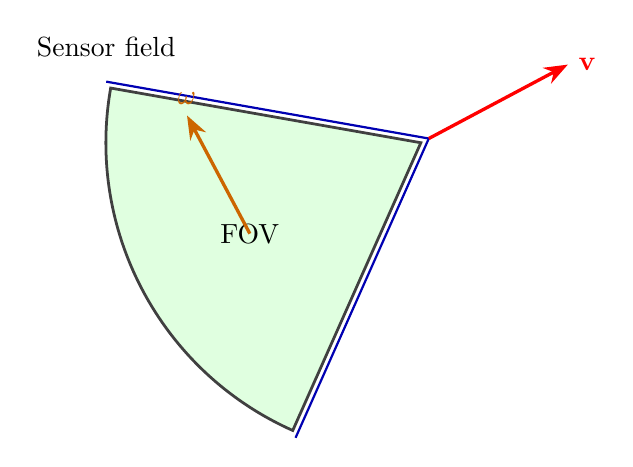
\begin{tikzpicture}[>=Stealth]
  \node[circular sector,circular sector angle=76,
    shape border uses incircle,shape border rotate=28,
    minimum width=34mm,minimum height=40mm,
    draw=black!75,fill=green!12,line width=1pt,outer sep=2pt] (field) at (0,0) {FOV};
  \draw[blue!70!black,thick] (field.sector center) -- (field.arc start);
  \draw[blue!70!black,thick] (field.sector center) -- (field.arc end);
  \draw[-{Stealth[length=3mm]},red,line width=1.2pt]
    (field.sector center) -- ++(28:20mm) node[right] {$\mathbf v$};
  \draw[-{Stealth[length=3mm]},orange!80!black,line width=1.2pt]
    (field.center) -- ++(118:17mm) node[above] {$\omega$};
  \node[above=2mm] at (field.arc start) {Sensor field};
\end{tikzpicture}
\end{document}
